\documentclass[a4paper, 12pt]{article}

\usepackage[left=14mm, top=23mm, text={183mm, 252mm}]{geometry}
\usepackage[utf8]{inputenc}
\usepackage[slovak]{babel}
\usepackage[hyphens]{url}
\usepackage{hyperref}
\usepackage{graphicx}
\usepackage{listings}
\usepackage{longtable}
\usepackage{float}
\usepackage{xurl}
\usepackage{tabularx}
\usepackage{caption}

\begin{document}

\begin{titlepage}
	\begin{center}
		{\Huge 
        \textsc{Vysoké učení technické v~Brně}\\[0.5em]}
		{\huge 
        \textsc{Fakulta informačních technologií}}\\
		\vspace{\stretch{0.382}}
		{\Large Mikroprocesorové a vestavěné systémy}\\[0.6em]
        {\LARGE \textbf{Rozpoznávanie znakovej abecedy a zobrazovanie na 7-segmentovom displeji typu flipdot}}
        \vspace{\stretch{0.618}}
	\end{center}
	{\Large 2024 \hfill 
    Michal Balogh (xbalog06) }
\end{titlepage}

\tableofcontents

\newpage


\section{Úvod}

Zadaním bolo využiť zaujímavý typ elektromechanického displeja typu flip-dots a demonštrovať jeho využitie. Na vypracovanie som mal k dispozícii displej s rozmermi 4 riadky, každý po 7 znakov. Základným zadaním bolo zobrazenie jednoduchých správ a meranej teploty a vlhkosti. Po splnení tohto zadania som vytvoril neurónovú sieť, ktorá rozpoznáva písmená znakovej abecedy. Tieto dáta sú potom zobrazované na displeji.

\section{Video k projektu}

Fungovanie projektu si môžete pozrieť vo videu na nasledovnom odkaze: \href{https://www.youtube.com/watch?v=IdzLrns7vJk}{YouTube video}.

\section{Vybavenie}

\subsection{7-segmentový displej typu flip-dots}

S displejom sa dá komunikovať pomocou prevodníka RS-485, rýchlosťou 57600 baudov. Znaky na displeji sa nedajú nastaviť jednotlivo, ale naraz pomocou dátového rámca, ktorý špecifikuje výrobca\footnote{\url{https://cdck-file-uploads-europe1.s3.dualstack.eu-west-1.amazonaws.com/arduino/original/4X/3/5/2/352c3c32d1ddcd251f45966920b16b53f3214f32.pdf}}:

\begin{verbatim}
+-------+----------+---------+----------------+-------+
| 0x80  | Command  | Address |      Data      | 0x8F  |
+-------+----------+---------+----------------+-------+
\end{verbatim}

Na začiatku je hlavička \texttt{0x80}. \( \texttt{Command} \) špecifikuje, ktorý typ displeja bude prijímať dátový rámec. Pre typ displeja, s ktorým som pracoval (4x7), je príkaz \texttt{0x83} – posiela 28 Bajtov dát a refreshne displej. Refresh znamená, že dáta sa rovno zobrazia na displeji. Adresu používam \texttt{0xFF} – čiže broadcast. Dáta sú o veľkosti 4x7 Bajtov. Jeden Bajt predstavuje 7 segmentov. Na konci je ešte päta \texttt{0x8F}.

Nastavenie jedného znaku je dané siedmimi bitmi. Na obrázku môžeme vidieť, ktoré bity nastavujú ktoré segmenty, a príklad, ako nastaviť nápis \texttt{PF 2024}.

\begin{figure}[H]
    \centering
    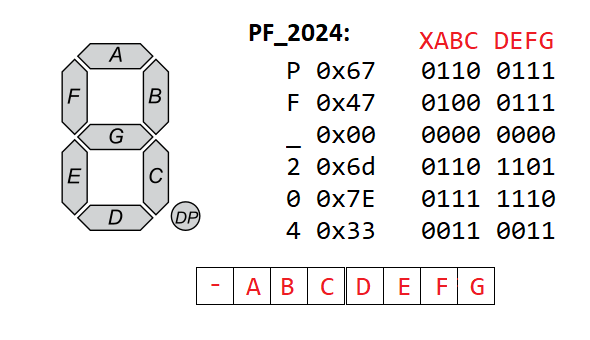
\includegraphics[width=0.7\textwidth]{segmentEncoding.png}
    \caption{Kódovanie segmentov}\label{fig:7seg}
\end{figure}

Na displeji nie je desatinná bodka, a teda MSB je ignorovaný a mal by byť nastavený na 0.

\subsection{Kombinovaný senzor na teplotu a vlhkosť DHT11}

Senzor DHT11 je jednoduchý kombinovaný senzor, ktorý meria teplotu v rozsahu 0 -- 50 stupňov Celzia s presnosťou ±1~°C a vlhkosť v rozmedzí 20 -- 90~\% s presnosťou ±4~\%. Existuje senzor DHT22 podobného druhu, ktorý by sa dal využiť na presnejšie merania, ale ja som mal k dispozícii tento.

Senzor má štyri vývody, z toho jeden je nezapojený, dva sú použité na napájanie v rozsahu 3~V až 5~V a jeden je dátový\footnote{\url{https://arduinoposlovensky.sk/projekty/dht11-a-dht22/}}.

\begin{figure}[H]
    \centering
    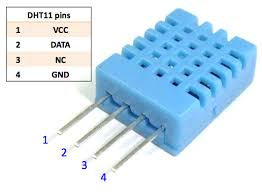
\includegraphics[width=0.5\textwidth]{dht11.jpg}
    \caption{DHT11 senzor}\label{fig:dht11}
\end{figure}

\subsection{Prevodník RS485}

Pre komunikáciu s 7-segmentovým displejom je použitý prevodník RS-485. Je to prevodník linky UART na sériovú linku RS485. Linka je poloduplexná\footnote{\url{https://techfun.sk/produkt/rs485-prevodnik-s-cipom-max485esa/}}. Linke treba okrem rýchlosti na 57600 baudov nastaviť aj ďalšie parametre: vypnúť paritný bit, nastaviť jeden stop bit a nastaviť 8 bitov na jeden Bajt. V jazyku C sa to dá nastaviť takto (knižnica \texttt{termios.h}):

\begin{verbatim}
tty.c_cflag &= PARENB; 
tty.c_cflag &= CSTOPB;
tty.c_cflag &= CSIZE;
tty.c_cflag |= CS8;
\end{verbatim}

Tento kód je implementovaný vo variante riešenia číslo 1, v súbore \texttt{./rpi4\_py\_c/serial\_com\_c/src/serial.c}.

\section{Varianty riešenia}

Postupne som skúšal rôzne riešenia a skončil som s troma rôznymi variantami:

\begin{itemize}
    \item Varianta 1: rpi4 C+Python
    \item Varianta 2: rpi4 Python
    \item Varianta 3: esp8266 C+Python
\end{itemize}

\subsection{Varianta 1: rpi4 C+Python}\label{var1}

Implementačná platforma pre túto variantu je Raspberry Pi 4. Celá implementácia varianty 1 je v priečinku \texttt{rpi4\_py\_c}. S touto variantou som začal tým, že som nastavil sériovú komunikáciu s displejom, vytvoril funkcie na vytvorenie správy a nastavovanie jednotlivých znakov pomocou indexovania do 2D poľa displeja (4x7) a mapovania na konštantné definované symboly (viď obr.~\ref{fig:7seg}). Vytvoril som si pár príkladov (\texttt{examples.c}), kde sa posielali konštantné správy, a na nich som otestoval funkčnosť pripojenia na displej a správny formát dátového rámca správy.

Druhá časť tejto varianty je implementovaná v Pythone. Najprv som vytvoril dataset pre rozpoznávanie znakovej reči. Využil som ASL dataset a modul \texttt{Hands} z frameworku \texttt{Mediapipe}. Pomocou skriptu \texttt{train/reduce\_dataset.py} som zredukoval počet obrázkov pre triedu v datasete na 200. Potom pomocou modulu \texttt{Hands} som z obrázkov datasetu extrahoval orientačné body z rúk. Konkrétne 21 bodov v 3D priestore a tie som uložil do \texttt{csv} súboru so 64 stĺpcami: 1 označenie znaku a 21\(\times\)3 (x,y,z) súradníc. Vytvorenie datasetu je v súbore \texttt{train/create\_hand\_landmarks\_dataset.py}. V súbore \texttt{train/ASL\_handm\_landmarks\_dataset.py} je vytvorená PyTorch \texttt{Dataset} trieda \texttt{ASLLandmarkDataset}. Samotný model je v súbore \texttt{train/gesture\_recognition\_model} a tréningový skript je v súbore \texttt{train/train.py}.

Natrénovaný model je použitý na inferenciu v skripte \texttt{rpi4\_py\_c/gesture\_recognizer\_py/main.py}. Tento skript načíta model, otvorí kameru a pomocou modulu \texttt{Hands} z \texttt{Mediapipe} získa orientačné body ruky. Tieto body sú potom použité na predikciu znaku. Tento skript komunikuje s programom v C cez socket. \texttt{gesture\_recognizer} posiela predikované znaky cez socket na program v C \texttt{serial\_com\_c}, ktorý posiela znaky na displej. \texttt{gesture\_recognizer} taktiež vizualizuje znaky a obraz kamery.

Program treba spustiť v dvoch termináloch. V jednom treba spustiť \texttt{main.py} a v druhom \texttt{main.c}.

\subsection{Varianta 2: rpi4 Python}

V tejto variante beží celý program v Pythone na Raspberry Pi 4. Celý program je v priečinku \texttt{rpi4\_py} a dá sa spustiť pomocou skriptu \texttt{main.py}. Tento skript podobne ako vo variante 1 načíta natrénovaný model, otvorí kameru a nastaví sériovú komunikáciu s displejom. Jediný rozdiel je, že dáta neposiela cez socket, ale priamo cez sériovú linku do displeja.

\subsection{Varianta 3: esp8266 C+Python – Finálna varianta}

Posledná varianta je implementovaná na platforme \texttt{ESP8266}. Implementáciu je možné nájsť v priečinku \texttt{esp8266}. Táto varianta je rozdelená na dve časti. Prvá časť je \texttt{server\_gestures} implementovaná v Arduine. Táto časť slúži ako server. Pomocou Wi-Fi modulu sa pripojí do siete a čaká na dáta od klienta na určitej IP adrese a porte. Dáta od klienta posiela na sériovú linku a tie sa zobrazujú na displeji. Sériová linka je pripojená na prevodník RS485 na dátových pinoch D2 (TX) a D3 (RX). Veľkou výhodou tejto varianty je, že klient je úplne nezávislý od servera a môže byť implementovaný na akejkoľvek platforme a posielať v podstate hocijaké dáta. V mojom prípade som už využil natrénovaný model na rozpoznávanie znakov a posielal som predikované znaky na server. Ale klient sa dá vymeniť za hocijaký iný program, ktorý bude posielať znaky na server a ten ich bude zobrazovať na displeji. Okrem toho, v tejto variante je upravený beh programu na \texttt{ESP8266}. Po pripojení do siete sa vypíše animovaná uvítacia správa \texttt{HELLO}. Následne sa môže program dostať do dvoch stavov: stav \texttt{IDLE} a stav \texttt{CONNECTED}. Začína v stave \texttt{IDLE} a čaká na pripojenie zariadenia na konkrétny port. V tomto stave zobrazuje na displeji čas, teplotu a vlhkosť. Teplotu a vlhkosť získava zo senzoru DHT11. Senzor je zapojený do dátového pinu D5. Po pripojení zariadenia sa prejde do stavu \texttt{CONNECTED}, ktorý je signalizovaný blikajúcim kurzorom a začne prijímať dáta od klienta a zobrazovať ich na displeji. Po ukončení spojenia prejde zase do stavu \texttt{IDLE}.

\section{Záver}

Projekt bol náročný na vypracovanie, ale keďže bol veľmi zaujímavý, išlo to dobre. Najzložitejšou časťou bolo vymyslenie štruktúry programu – komunikácie medzi jednotlivými časťami. Najspokojnejší som s poslednou variantou, kde je spracovanie dát veľmi flexibilné a displej sa dá využiť na zobrazovanie hocijakého textu aj v iných projektoch. Okrem toho ďalšou zložitejšou časťou bolo nastavenie sériovej komunikácie s displejom a vytvorenie dátového rámca podľa špecifikácie. Na projekte som strávil vyše 40 hodín.

\subsection*{Autoevaluácia:}
\begin{itemize}
    \item \textbf{E}: 2b – keďže zadanie som si vymyslel sám, chcel som ho dotiahnuť do stavu, ktorý sa mi bude páčiť, a preto som aj vytvoril 3 rôzne varianty
    \item \textbf{F}: 5b – hlavne posledná varianta spĺňa všetky požiadavky zadania a okrem toho má rôzne bonusy, ako napríklad zaujímavé animácie
    \item \textbf{Q}: 2b
    \begin{itemize}
        \item Užívateľská prívetivosť: užívateľ sa môže pripojiť buď so svojím programom a na jednoduché rozhranie posielať znaky na displej, alebo môže použiť môj program na rozpoznávanie znakov a posielať predikované znaky na displej, ktoré aj vidí na obrazovke, kde sa zobrazuje výstup
        \item Spôsob implementácie: implementácia je rozdelená na dve časti, server a klient, ktoré sú nezávislé a komunikácia medzi nimi prebieha cez Wi-Fi
    \end{itemize}
    \item \textbf{D}: 3b
    \begin{itemize}
        \item Úvod do problému: Myslím si, že jasne popisujem, čo je cieľom projektu
        \item Popis riešenia: Do detailu popisujem všetky 3 varianty a ich implementáciu
        \item Zhodnotenie: Zhodnotenie je podrobné a obsahuje všetky potrebné časti
    \end{itemize}
    \item \textbf{P}: 2b
    \begin{itemize}
        \item Verím, že projekt odprezentujem dobre :) a prezentácia projektu samotného je pekná vizuálna, interaktívna a zaujímavá
    \end{itemize}
    \item \textbf{SUM}: 14b
\end{itemize}

\section*{Zdroje}


\begin{itemize}
    \item \url{https://arduinoposlovensky.sk/projekty/dht11-a-dht22/}
    \item \url{https://techfun.sk/produkt/rs485-prevodnik-s-cipom-max485esa/}
    \item \url{https://papouch.com/prevodniky/rs485/}
    \item \url{https://learn.microsoft.com/en-us/windows/wsl/connect-usb}
    \item \url{https://blog.mbedded.ninja/programming/operating-systems/linux/linux-serial-ports-using-c-cpp/}
    \item \url{https://www.kaggle.com/datasets/grassknoted/asl-alphabet?\
    select=asl_alphabet_test}
    \item \url{https://randomnerdtutorials.com/getting-started-with-esp8266-\
    wifi-transceiver-review/}
    \item \url{https://randomnerdtutorials.com/esp32-ntp-client-date-time-\
    arduino-ide/}
    \item \url{https://projecthub.arduino.cc/arcaegecengiz/using-dht11-12f621}
\end{itemize}


\end{document}